\section{Confidetnial Services}
In this section I present two Confidential Cloud Services. The first one is the Confidential Consortium Framework (CCF)~\cite{Howard} and the second one is Nimble~\cite{Nimble}. They both provide a structure to guarantee the CIA properties, but have some differences in their design, especially when it comes to rollback attacks. Nimble is specialized in detecting rollback attacks while CCF is a whole framework that can also be used for multiparty applications.
\subsection{CCF}
The basic idea of CCF is that an untrusted host exists and one or more untrusted users can access different replicated nodes that are responsible for the remaining communication. One of these nodes is the primary. Users can connect to any node and the specific request is either being forwarded to the primary or handled by the node itself. Operations that do not have the obligation to be handled in the primary are read-only requests. If this node fails the user can be connected to another node, if the primary fails there is a primary election that selects a new primary with certain voting criteria. The primary also periodically sends signature transactions. These are transactions that confirm that there were no malicious changes to the code and thus guarantee the integrity of CCF. Transactions (i.e. user requests) are provided via a merkle tree, where each transaction is a hash value. Every two nodes in the merkle tree are combined with a hash function to a new node. On top of the merkle tree is the merkle root, which is the value that is used for the signature transaction. %maybe figure
 Providers only need to implement the application logic and make sure to have all necessary endpoints, so that CCF can handle these. Users then only have to access the specific endpoints to use the application.  In Figure~\ref{ccf} the structure of one node is described. The application logic gets the data from the Key-value-store which gets the data from the Consensus. %TODO: what is the Consensus
  The Transaction Handler stores every signature transaction in an append-only ledger that is redundant in every other node and the persistent storage. Performing the application logic inside a TEE is fundamental for the confidentiality and the integrity, replicating the transactions is necessary for the high availability. The ledger is stored outside the TEE what leads to certain problems that are discussed in~\ref{challenges:ccf}.
\begin{figure}[t]
	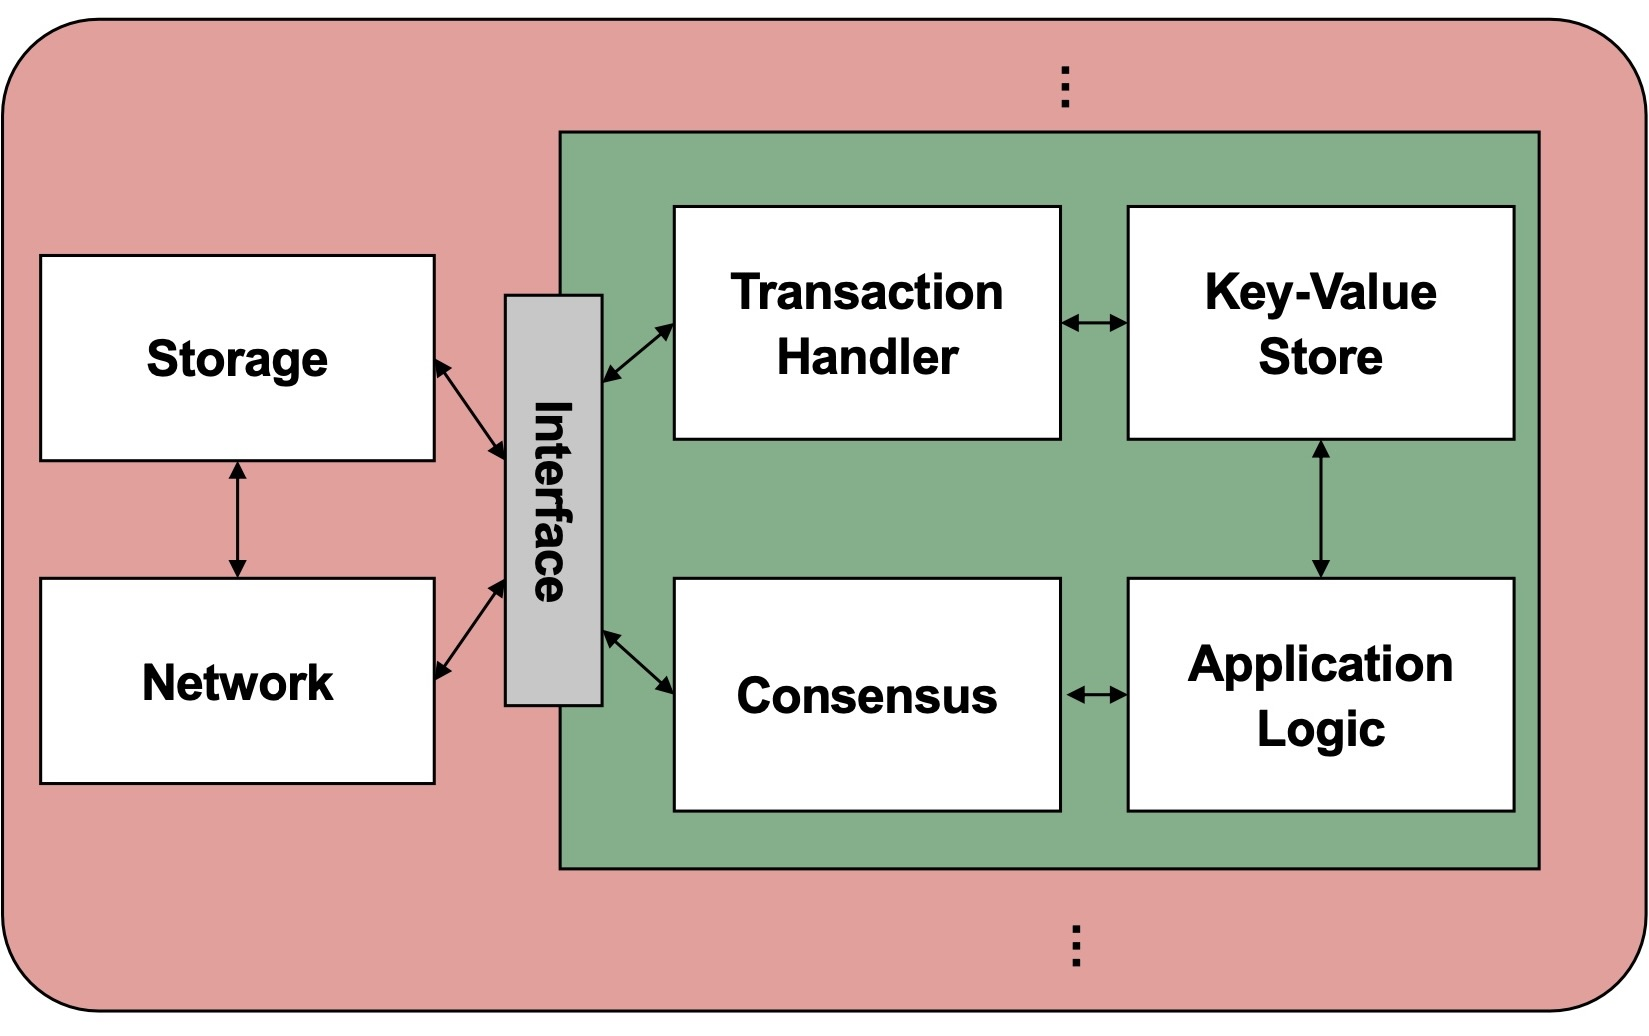
\includegraphics[scale=0.14]{pictures/ccf}
	\caption{Each node consists of a TEE, the untrusted host, and an interface between the host and the TEE. The TEE consists of a Key-value store, the Consensus, the Transaction Handler and the specific Application logic.The storage and the network are placed outside the TEE.}
	\label{ccf}
\end{figure}
\subsection{Nimble}
Nimble also tries to ensure the requirement of the CIA triad, but has the focus of preventing rollback attacks.
Nimble has three important goals, (1) ensure linearizability, (2) having a small Trusted Computing Base (TCB) and (3) to guarantee liveness of the cloud service. Therefore the authors differ between two main properties:
\begin{itemize}
	\item \textbf{Safety} means that it must be ensured that every data that can be accessed must be the current data and must not be an older version. This property is enabled via TEEs. In the CIA triad this would be Confidentiality and Integrity.
	\item \textbf{Liveness} is the High Availability property of the CIA triad. This has not to be ensured via a TEE, because liveness can be easily taken away even in an TEE, and can be handled outside what simultaneously makes the TCB smaller.
\end{itemize}
	To guarantee liveness Nimble stores the data redundantly via state machine replication. To guarantee safety the state of each replicated node is apended to a ledger which is stored as a hash chain in an existing storage provider. Inside each TEE there is a trusted state machine that is called endorser. The endorser stores the tail of the hash chain for each ledger. So if data is read from the ledger it can be compared with the endorser. If it is not the same then a rollback attack did happen or the system failed before the endorser could store the tail of the hash chain. As there are replicated endorsers in nimble, it can still guarantee liveness, if endorsers fail, as long as there is a majority of working endorsers. To guarantee liveness even if a majority of endorsers fails, Nimble implements reconfiguration, which is described in~\ref{reconNimble}. 
\begin{figure}[b]
	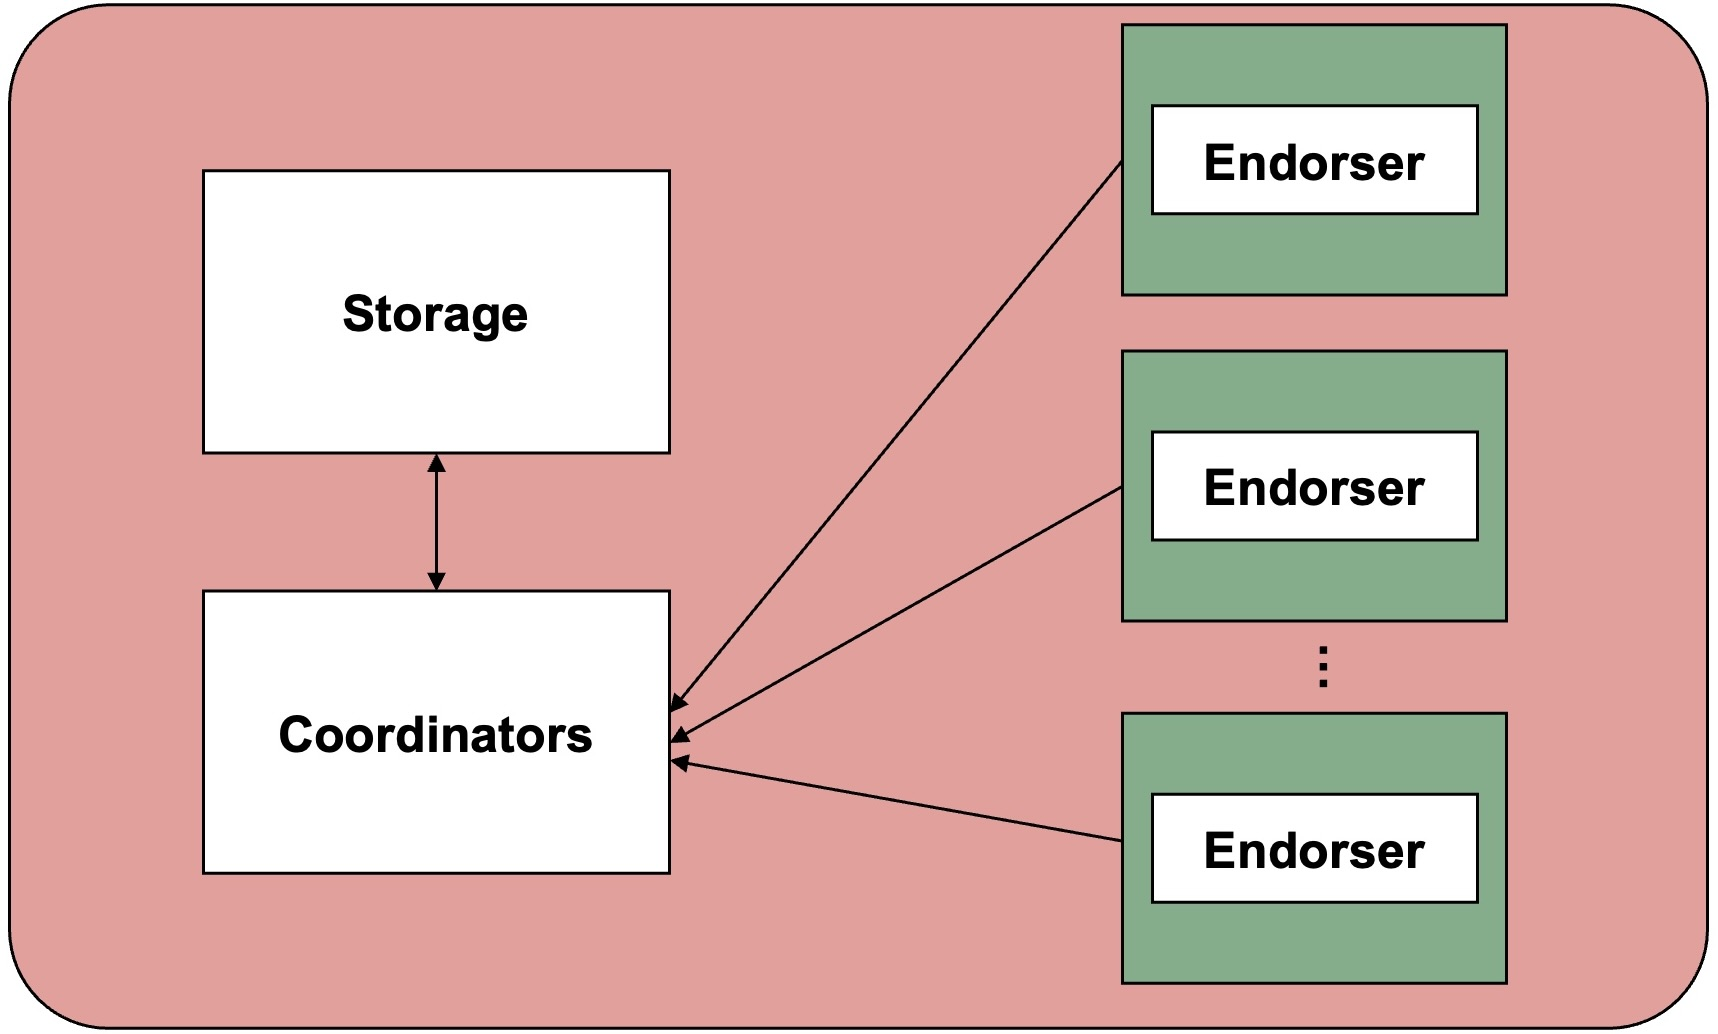
\includegraphics[scale=0.12]{pictures/nimble}
	\caption{Each node consists of a TEE. Inside the TEE there is the Endorser that saves the tail of the ledger.}
	\label{nimble}
\end{figure}
